\section{Les données}
  Dans un projet complexe comme celui de Conquêtes, le nombre de données à traiter est considérable c'est pourquoi nous avons du commencer le projet par la schématisation 
  des données puis leur réalisation.
  Nous comptons au total, 28 classes de données répartis autour de plusieurs catégories :
  \begin{itemize}
    \item Le joueur
    \item Bâtiments
    \item Territoires
    \item Troupes
  \end{itemize}
  
  \subsection{Les joueurs}
    Pour les joueurs nous avions besoin de différentes données :
    \begin{itemize}
      \item Son stock de ressources \\
	Par simplification nous avons implémenté un seul type de ressource. Mais la gestion de plusieurs ressource est déjà effective (utilisation d'un HashMap).
      \item Alliés \\
	Les alliés sont représentés sous forme de graphes. Un joueur peut-être alliés à différents joueurs sans que ceux ci soit forcément alliés.
      \item Informations pratiques \\
	Le joueur possède aussi un nom et un numéro afin de pouvoir rapidement le reconnaitre.
    \end{itemize}
  
  \subsection{Les batiments}
    Nous avions besoin de plusieurs type de bâtiment ayant chacun une fonctionnalité (Militaire, Production de ressources, Défenses) ainsi que d'un bâtiment général pour la capitale
    qui implémente toutes les fonctionnalités.
    Nous avons donc une classe mère qui nous permettra de gérer chaque bâtiment de la même manière quel que soit sa spécification. Ensuite chacune de ses classes filles implémente
    une ou plusieurs interface correspondant à leur spécification. La capitale implémente donc les trois interfaces.
    \vspace{0.5cm}
    Chaque bâtiment possède :
    \begin{itemize}
      \item Un nombre de tours qu'il faudra au bâtiment pour être opérationnel après que le joueur ai lancé sa construction
      \item Un coût en ressource pour pouvoir construire le bâtiment
      \item Un ou plusieurs attributs spécifique à sa ou ses spécifications \\
	Chaque spécifications rajoute un ou plusieurs attributs au batiment. Des unités en construction pour les batiments militaires, des pourcentages d'augmentation de ressources pour les
	batiments de resources ou des statistiques de défenses améliorées pour les batiments de défenses
    \end{itemize}
    
  \subsection{Territoires}
    Les territoires sont les données qui composent notre map. Nous avons choisi de représenter cette map sous forme de graphe. C'est à dire que nous ne voyons pas la carte comme un tableau de
    territoire mais comme un ensemble de territoires voisins. \\
    Nous avons défini aussi plusieurs types de territoires (Plaine, Montagne etc...) gérés par une classe mère comme les batiments. \\
    Chaque territoire peut être représenté comme un hexagone (il a six voisins). \\
    Un territoire peut-être définie comme non traversable ou non. \\
    Un territoire traversable peut-être définie comme une capitale.
    \vspace{0.5cm}
    Chaque territoire a :
    \begin{itemize}
      \item Un possesseur (Vaut null si le territoire est neutre)
      \item Un  batiment de n'importe quel type (sauf la batiment des capitales ne pouvant être que sur une capitale). Ce batiment est soit construit soit en construction soit non construit.
      \item Des troupes d'une même alliance (celle du possesseur)
      \item Six territoires voisins
      \item Un stock et une production de ressources
    \end{itemize}

  
  \subsection{Troupes}
	Nous avons réalisé plusieurs types de troupes afin de varier les techniques d'assauts et de défenses. Chaque troupes peut-être composée de plusieurs soldats d'un même type. \\
	Chaque troupe a \\
    \begin{itemize}
      \item Un possesseur
      \item Une valeur d'attaque (en fonction du nombre/type de soldat)
      \item Une valeur de défense (en fonction du nombre/type de soldat)
      \item Un nombre de tours pour être formé (en fonction du type de soldat)
      \item Le coût nécessaire en ressource (en fonction du type de soldat)
    \end{itemize}
  
  
  \section{Le moteur}
    Le moteur est la partie calculatoire de notre programme. C'est lui qui va construire la partie et la faire avancer en fonction de ce que lui enverra l'interface graphique.
    Nous avons répartis la conception du moteur selon différentes catégories :
    \begin{itemize}
      \item La génération et le controle de la map
      \item La gestion des différentes phases de jeux
      \item La gestion des joueurs et leurs actions possibles
      \item Enfin la boucle de jeu qui initialise et coordonne tout ces éléments
    \end{itemize}

  
    \subsection{La Map}
      Cette partie va permettre de générer le graphe de territoire en fonctions de plusieurs paramètres. \\
      Ce graphe est toujours généré de la même manière, seuls le placement des types de territoires sera fait en fonction des différents types de maps. \\
      Les map possèdent un itérator propre pour faciliter leur parcours. \\
      
      \subsubsection{Map aléatoire}
	La map aléatoire génère des territoires de manières complètement aléatoires. Elle prend deux paramètres :
	\begin{itemize}
	  \item Le nombre de ligne de la map
	  \item Le nombre de colonne de la map
	\end{itemize}
	\vspace{0.5cm}
	Représentation d'une map aléatoire : 
	
	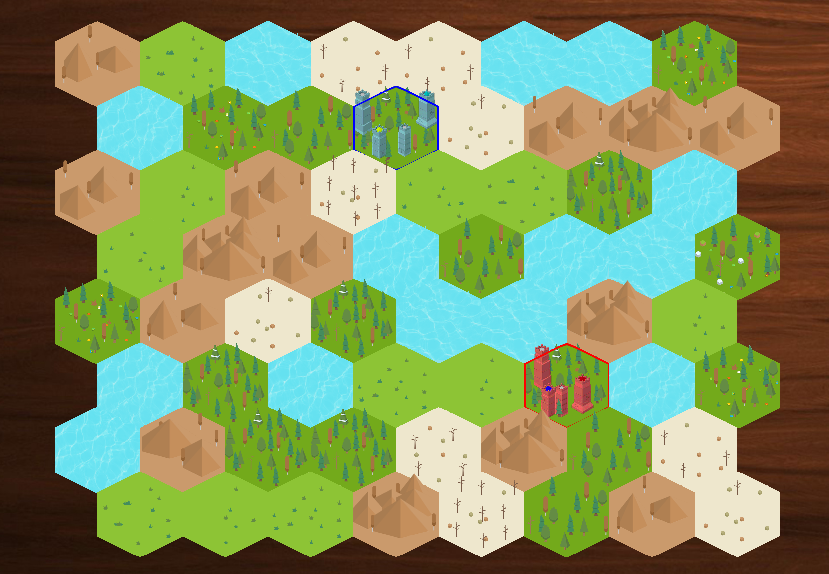
\includegraphics[scale=0.7]{map/random.PNG}

      
      \subsubsection{Map procédurale}
	La map procédurale va générer les différents types de territoires sous forme de biomes. C'est à dire que les territoires ne seront plus placés sans ordre précis, mais les
	territoires de mêmes types vont avoir tendance à se rassembler. Le placement des biomes est lui aléatoire. \\
	Elle prend quatre paramètres :
	\begin{itemize}
	  \item Le nombre de ligne de la map
	  \item Le nombre de colonne de la map
	  \item La taille minimum d'un biome
	  \item La taille maximum d'un biome
	\end{itemize}
	\vspace{0.5cm}
	
	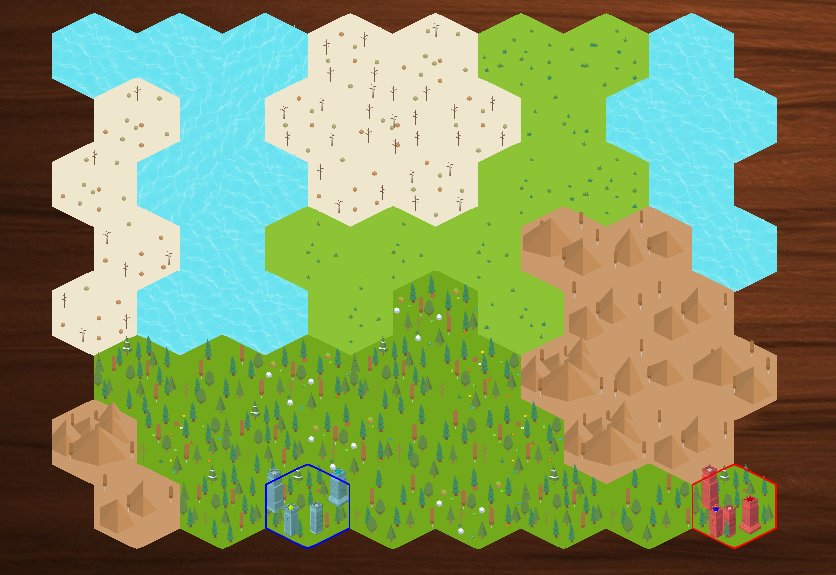
\includegraphics[scale=0.7]{map/procedural.PNG}
	
      \subsubsection{Map générée par le joueur}
	Voir la partie éditeur de la section "graphique"
    
    \subsection{Les phases de jeux}
      Le système de jeu se divisent en plusieurs tours. Chaque tour est divisé en deux phases
      
      \subsubsection{La phase de gestion}
	C'est la phase ou les joueurs vont pouvoir faire leurs différentes actions. Il y a une phase de gestion par joueur par tour.
	
      \subsubsection{La phase de combat}
	Elle commence quand toutes les phases de gestions sont terminées. \\
	On va regarder touts les territoires en conflits, c'est à dire ou des unités d'alliances différentes sont présentes. \\
	On fait le rapport des forces et on détermine le vainqueur (celui qui a le plus de troupes). En cas de forces égalitaires, le vainqueur est tiré au hasard.
    
    \subsection{Les joueurs}
      On peut séparé deux types de joueurs, les joueurs humains et les IA. Ils seront traités de la même façon dans le jeu, seul la manière dont ils font leurs actions changent.
      
      \subsubsection{Les joueurs humains}
	Ils font leurs actions à partir de l'interface graphique pendant les phases de gestion.
    
      \subsubsection{Les IA}
	Leurs actions est calculés par le moteur pendant leurs phases de gestions. On peut définir deux IA de niveaux différentes :
	\begin{itemize}
	 \item \underline{L'IA défensive} : \\
	  C'est une IA basique. Elle va juste chercher à établir des défenses autour de sa position pour empecher l'ennemi de l'atteindre et s'expendre ainsi.
	 \item \underline{L'IA agressive} : \\
	  Cette IA a un comportement qui s'adapte en fonction des actions de(s) adversaire(s). Pour cela nous avons définis des états dans lequel l'IA peut se trouver.
	  Chaque état mène vers un ou plusieurs états en un nombre de tour défini jusqu'à arriver à l'état final recherché (la destruction de la capitale ennemi). \\
	  L'IA va donc appliquer l'algorithme de dijkstra qui est un algorithme très utilisé en pathfinding. Elle va donc pouvoir décider seule des meilleurs actions à faire.
	\end{itemize}

      
      \subsubsection{Les actions possibles}
	Les joueurs peuvent faire plusieurs actions par tour de jeux. En cas d'action impossible, on renvoie une erreur correspondant à l'action. \\
	Les actions possibles sont :
	\begin{itemize}
	 \item Créer/Détruire/Accepter/Rejetter une alliance.
	 \item Créer un batiment sur un territoire vide.
	 \item Créer une troupe dans un batiment militaire
	 \item Déplacer une troupe
	 \item Finir son tour
	\end{itemize}

  
    \subsection{La boucle de jeu}
      La boucle de jeu s'éxécute de la même façon à chaque tour. Elle va mettre en relation tout les éléments ci-dessus :
      \begin{itemize}
       \item On commence par parcourir la map pour produire les ressources de chaques territoires et les donner à leurs possesseurs, pour faire avancer les unités/batiments en constructions etc...
       \item Ensuite on lance la phase de gestion de tout les joueurs et on attend que chaque joueur ai fini son tour
       \item Quand tout le monde a fini son tour, on lance la phase de combat.
       \item Enfin, on regarde si c'est la fin du jeu. Si ce n'est pas le cas on reboucle, sinon on stop et on annonce le vainqueur.
      \end{itemize}
      
    \subsection{Fin du jeu}
      La fin du jeu est déterminée quand il ne reste plus qu'un seul joueur en jeu (Quand il possède donc toutes les capitales). Ce joueur est déclaré vainqueur.
  
  \section{L'interface graphique}
  
  Le graphique est un des pôles les plus important dans la réalisation d'un jeu vidéo, dans notre jeux conquêtes, il a fallut dessiner de nombreux éléments graphiques ainsi que de nombreuses classes graphiques.
  \\
  \\
  \subsection{Les éléments graphiques}
  Au niveau des éléments graphiques, nous pouvons lister :
  \\
  \begin{itemize}
    \item Boutons
    \item Police d'écritures
    \item Images de fond
    \item Textures des territoires
    \item Menu
    \item Skin des soldats
    \item Skins des batiments
    \item Fenêtre de dialogue\\
  \end{itemize}
  
  La police d'écriture du jeu, est la fameuse Korinna, en libre droit d'utilisation, elle fut désigné en 1974, celle-ci est encore utilisé par Disney, Capcom ainsi que de nombreux journaux.
  Une partie des éléments graphiques (arbres, boutons, etc) ont été réalisé par Kenney, un game designer hollandais qui publient des pack de sprites pour des développeurs de jeux vidéos, il va de soi que les packs que nous avons utilisés sont libre de droits.
  Pour la réalisation et l'assemblage des éléments graphique, nous avons utilisé exclusivement GIMP sous Windows, ce qui nous à permis d'adapter les divers éléments graphiques à nos besoin.
  
  \subsection{Les classes graphiques}
Au niveau des classes générant un rendu graphique, nous les avons mis dans un dossier screen, et elles commencent toutes par Gui.
\\
\\
  Voici la listes avec leur descriptions respectives :
  \\
  \begin{itemize}
    \item GuiEditor
      GuiEditor nous permet d'accéder au mode éditeur. Le mode éditeur nous permet de créer notre propre map avec les types de territoires, capitales etc.\\
    \item GuiGame
      GuiGame est la classe la plus importante de notre projet, en effet, celle-ci gère l'affichage complet du jeux.\\
    \item GuiHelp
      GuiHelp est une page d'aide pour l'utilisateur accessible via le bouton aide dans GuiGame.\\
    \item GuiLoading
      GuiLoading nous affiche la page de chargement de parties.
    \item GuiMenu
      GuiMenu gère l'affichage et les interactions de l'utilisateur avec le menu principal du jeu.\\
    \item GuiResult
      GuiResult s'affiche en fin de partie, celle-ci annonce la fin de la partie et propose au joueur de rejouer.\\
    \item GuiSettings
      GuiSettings comme son nom l'indique permet d'accéder aux menu de réglages du jeux.\\
    \item GuiStream
     GuiStream est l'interface qui permettant de rediriger les messages d'erreurs vers la  fenêtre graphique.\\
  \end{itemize}
  
  \subsection{Les extensions}
    Nous avons dans notre projet réussi à réaliser deux extensions du cahier des charges :
    \subsubsection{Mise en place des langues}
      Nous avons mise en place un système de fichier de localisations. Il nous est donc possible de changer de langue n'importe quand pendant le jeu. Pour l'instant les langues gérées sont
      l'anglais et le français mais il nous est très simple d'en rajouter.
      
    \subsubsection{Mise en place du réseau}
      Nous avons aussi mis en place une surcouche réseau "Serveur/Client" dans notre jeu. Le serveur communique avec le moteur et le client avec l'interface graphique.
      Il est donc possible de jouer jusqu'à 8 joueurs en même temps sur 8 postes différents. Cela accèlère la vitesse des parties